\chapter{Model Predictive Control}
\label{chap:chap3}

In questo capitolo si approfondisce il lavoro principale di questa tesi che,
come anticipato in precedenza, è stato lo studio e l'implementazione di un sistema
di \textit{path tracking} che permettesse al veicolo di seguire
un percorso -- composto da una serie di \textit{waypoint} equidistanti -- mediante 
un tracking preciso della traiettoria di riferimento, eventualmente tentando anche di 
ridurre i tempi di completamento di un giro su specifici circuiti da corsa.

Per raggiungere questo scopo, si è scelto di realizzare 
\textit{Model Predictive Control} (\textit{MPC}), 
un controller all’avanguardia che, generalmente, viene progettato per 
automatizzare un sistema di \textit{sensori} e \textit{attuatori},
come sistemi energetici industriali o robotici.
Tra l'altro, anche Ayrton Senna, uno dei più grandi piloti di Formula 1 
di tutti i tempi, andava ad applicare una strategia simile a \textit{MPC}, attraverso la 
\textit{tecnica dell’acceleratore}. In pratica, Senna aveva un modello mentale del 
comportamento del turbocompressore e, in modo predittivo, cercava di massimizzare 
l’accelerazione in uscita da una curva~\cite{f1tenthcoursel13}.

Le metodologie basate su \textit{MPC} rappresentano la soluzione principale alla base di 
diversi controller per veicoli da corsa autonomi che sono stati implementati su veicoli reali~\cite{Betz2022}.
Più precisamente, si tratta di una strategia di controllo che sfrutta un 
determinato \textit{modello della dinamica dell’ambiente} e, rispettando una serie di 
\textit{vincoli}, è in grado di controllare un dato processo. 
Il modello deve essere adeguato al sistema o processo da controllare poiché uno
dei vincoli da soddisfare è proprio il modello. Pertanto, esso viene utilizzato per 
prevedere il comportamento futuro con l'\textit{obiettivo} di trovare l'input di controllo 
\textit{ottimale}, che deve essere applicato per un certo \textit{orizzonte temporale} scelto.

Nel contesto di questa tesi e di \textit{F1TENTH}, lo scopo di \textit{MPC} è generare,
per $N$ passi futuri, controlli di input validi che guidino il veicolo il più vicino 
possibile alla traiettoria di riferimento, garantendo al contempo prestazioni stabili anche a 
velocità sostenute.
Come accennato, \textit{MPC} è in grado di gestire i vincoli del sistema, cosa che non è 
possibile con un metodo reattivo come il \textit{PID}. Quest'ultimo, infatti, è un sistema
di tipo \textit{SISO} (\textit{Single Input, Single Output}), in grado di gestire
solo un singolo input $e(t)$ e generare un singolo output $u(t)$. Un esempio può essere 
l'avere come input l'errore dell'angolo di sterzata e come output il calcolo del nuovo angolo di sterzata.

Quindi, tra i due, conviene adottare \textit{MPC}, anche perché le dinamiche dell’ambiente
possono cambiare nel tempo e \textit{MPC} offre un modo semplice per stimare tali dinamiche e 
adeguarsi correttamente. Al contrario, \textit{PID} non è adatto per i sistemi la cui
dinamica cambia frequentemente, perché potrebbe essere necessario modificare 
continuamente i valori dei \verb|gain| di controllo per ottenere il comportamento
desiderato, rischiando comunque di imbattersi in un \textit{overshoot}.
Inoltre, a differenza di \textit{PID}, \textit{MPC} è dotato di un vettore di 
\textit{input di controllo} e di un vettore di \textit{stato}, dunque è un sistema di tipo 
\textit{MIMO} (\textit{Multi-Input, Multi-Output}), che consente cioè a più input di variare l’output del sistema.

Un'alternativa di tipo \textit{MIMO} a \textit{MPC} è \textit{LQR} 
(\textit{Linear Quadratic Regulator}), una versione senza vincoli 
e più semplice di MPC~\cite{f1tenthcoursel13}, che però ha i seguenti limiti:
\begin{enumerate}
    \item non è in grado di gestire dei vincoli;
    \item può generare input di controllo impraticabili per il robot, come un angolo di sterzata di $\frac{\pi}{2}$.
\end{enumerate}
\textit{MPC} risulta quindi essere un controllore che permette di soddisfare:
 \begin{enumerate}
     \item vincoli di \textit{sicurezza}, come velocità, accelerazione e limiti del percorso;
     \item vincoli \textit{fisici}, come mantenere una traiettoria possibile per la dinamica dell'auto.
 \end{enumerate}

 % Valutare se inserire questa img:
%https://docs.google.com/presentation/d/1QBXVAaRjFa0_fBHOmTFo2AHS1nvde_nONzNAGvCgCxM/edit#slide=id.g21997f8dc71_0_142

\section{Struttura}
Dopo aver analizzato le problematiche di altri metodi e aver introdotto \textit{MPC}, si vuole 
comprendere come controllare all'ottimo un sistema.
Infatti, il primo passo per impostare \textit{MPC} è definire il problema di controllo ottimale
da risolvere, che è caratterizzato dalle seguenti componenti:
\begin{enumerate}
    \item il \textit{modello} della dinamica del sistema, per prevedere il comportamento futuro.
    \textit{Esempio}: dinamica del veicolo;
    \item la \textit{funzione obiettivo} da minimizzare. \textit{Esempio}: \textit{cross-track error} e/o tempo di un giro;
    \item i \textit{vincoli} da rispettare all'interno del sistema. \textit{Esempio}: limiti della velocità, della sterzata, ecc.
\end{enumerate}
Pertanto, si tratta di un problema di \textit{ottimizzazione convessa} con vincoli e ciò 
che si vuole risolvere è la sequenza $[x_0 \ ... \ x_N \ \ \ \ u_0 \ ... \ u_N]^T$, composta da:
\begin{enumerate}
    \item azioni di controllo, indicate come $u$;
    \item stati previsti, indicati come $x$.
\end{enumerate}
Come anticipato, \textit{MPC} si prefigge di controllare un sistema risolvendo iterativamente un 
problema di ottimizzazione che sia in grado di prendere in considerazione un modello e dei vincoli fisici. 
Il controllore ha il compito di minimizzare una certa funzione obiettivo, detta anche di costo, 
attraverso la simulazione degli stati futuri, a partire da quello attuale e dalle variabili di 
controllo, secondo uno specifico modello del sistema.
Questi stati sono delimitati dai vincoli dati a \textit{MPC} in modo che non vengano raggiunti stati indesiderati e/o non praticabili. 
Le variabili di controllo possono quindi essere scelte in 
modo che gli stati generati soddisfino la funzione di costo. 

Il punto nel futuro fino al quale simula viene determinato da un \textit{orizzonte} di previsione 
finito: per un orizzonte più ampio il tracciamento risultante sarebbe certamente più fluido, 
ma anche più pesante a livello computazionale.
Le variabili di controllo calcolate possono quindi essere utilizzate come attuazione per il 
sistema controllato in quell'istante di tempo~\cite{racelinecontrol}.

\begin{figure}[H]
    \centering
    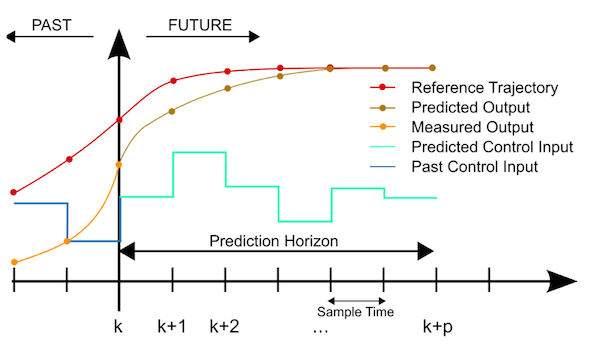
\includegraphics[scale=0.7]{images/mpc_prediction.png}
    \caption{Diagramma che mostra il lavoro 
    svolto da \textit{MPC}, differenziando tra 
    \textit{passato} e \textit{futuro} (con un certo orizzonte)~\cite{mpschema}.}
    \label{fig:fig8} % etichetta utilizzata per riferisi all'immagine
\end{figure}

Nella Fig.~\ref{fig:fig8} si può osservare
che la linea azzurra in basso è l'attuazione, 
un input di controllo discreto, mentre in alto 
si trovano sia la traiettoria di riferimento 
che quella futura prevista.
Il controllore prenderà in considerazione lo stato rilevato del sistema e 
ottimizzerà una sequenza di controllo ideale, 
in base alla funzione obiettivo definita.

Dunque, il problema di ottimizzazione con vincoli alla base di \textit{MPC} si può 
definire come la minimizzazione del costo di una traiettoria che sia praticabile per la
dinamica del sistema e che non violi i vincoli imposti. Si riporta di seguito un \textit{setup} 
generale di questo problema:
\[
\begin{aligned}
U_t^*(x(t)) := \min_{U_t} &\sum_{k=0}^{N-1} q(x_{t+k}, u_{t+k}) \\
\text{subject to } & x_t = x(t) & \quad & \text{misure} \\
& x_{t+k+1} = Ax_{t+k} + Bu_{t+k} & \quad & \text{modello del sistema} \\
& x_{t+k} \in \mathcal{X} & \quad & \text{vincoli dello stato} \\
& u_{t+k} \in \mathcal{U} & \quad & \text{vincoli degli input} \\
& U_t = \{u_t, u_{t+1}, \ldots, u_{t+N-1}\} & \quad & \text{variabili di ottimizzazione}
\end{aligned}
\]
Si specifica che con $k = 0$ si intende il time-step corrente, mentre con $k = N-1$ si fa 
riferimento al time-step antecedente alla fine della finestra dell'orizzonte temporale. 
Si discuterà maggiormente del tema nelle sezioni successive, entrando nello specifico di ciascuna 
componente del problema di ottimizzazione.

\subsection{Receding Horizon Control}
Alla base del funzionamento di \textit{Model Predictive Control} c'è il concetto di orizzonte finito, definito in letteratura come \textit{Receding Horizon Control}. 
Questo indica che, dopo che è stata applicata l'attuazione, viene calcolata una nuova serie di 
variabili di controllo per il nuovo stato del veicolo. 
\begin{figure}[H]
    \centering
    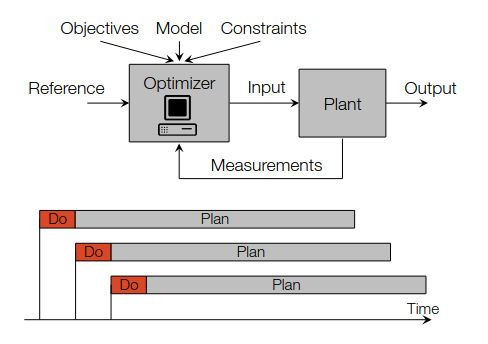
\includegraphics[scale=0.6]{images/mpc_horizon.png}
    \caption{Struttura di \textit{MPC con Receding Horizon Control}, in cui si pianifica per una 
    certa finestra di tempo~\cite{f1tenthcoursel13}.}
    \label{fig:fig9} % etichetta utilizzata per riferisi all'immagine
\end{figure}
Come si può osservare dalla Fig.~\ref{fig:fig9}, ciò viene reiterato in modo da aiutare il 
controllore nella gestione di comportamenti inaspettati.
Il vantaggio principale è rappresentato dal fatto che, 
applicando continuamente gli input di controllo ottimali, 
il sistema può essere portato verso un riferimento 
desiderato -- come una traiettoria ottima da seguire -- 
che viene raggiunto quando la funzione obiettivo risulta minimizzata.

Per progettare un controllore con queste caratteristiche, il sistema deve essere di tipo 
\textit{closed loop}, cioè deve includere un meccanismo di feedback in cui le variabili di 
controllo $u$ vengono calcolate in base all'errore tra gli stati di riferimento $x_{r e f}$ e gli stati simulati $x$.
Inoltre, l’orizzonte finito consente di avere un problema di ottimizzazione trattabile 
computazionalmente, in contrapposizione al controllo dell’orizzonte infinito 
(con un sistema \textit{``open loop''}), che risulterebbe impraticabile poiché 
considererebbe tutto l'ambiente -- il circuito in questo contesto -- e non più solo una parte di esso.

Più precisamente, i passi dell’\textit{MPC} con orizzonte finito sono i seguenti~\cite{mpcpeters}:
\begin{enumerate}
    \item Ottenere lo stato corrente $x(t)$;
    \item Calcolare, per una determinata finestra di pianificazione 
    temporale $N$, la sequenza di input di controllo ottimale: 
    $U^*_{t} = \{u^*_{t},\dots, u^*_{t+N-1}\}$;
    \item Applicare solo il primo input di controllo $u^*_{t}$;
    \item Ripetere per ripianificare.
\end{enumerate}
L'intuizione fondamentale è che, invece di applicare l'intera sequenza di input calcolata, si 
applichi solo il primo input ottimale per poter istantaneamente misurare lo stato risultante del veicolo. 
In questo modo si riescono a considerare preventivamente gli errori poiché viene introdotto un
feedback grazie alla successiva ripianificazione.

È presente un trade-off nella scelta dell'orizzonte di pianificazione $N$: idealmente, se ne 
vorrebbe avere uno breve che consideri pochi istanti temporali, risultando anche più leggero; 
tuttavia, con un orizzonte troppo ridotto la traiettoria pianificata potrebbe non tenere conto del 
comportamento futuro del sistema, portando il controllore a intraprendere azioni di controllo 
miopi -- ad esempio, mantenere un'accelerazione elevata in prossimità di una curva che non è stata rilevata.
D'altro canto, un orizzonte che guarda troppo in avanti renderebbe impegnativo il raggiungimento
di soluzioni precise, sia per ciò che riguarda la funzione di costo che per il rispetto dei vincoli.

\section{Modello}
Per poter formulare un problema di controllo ottimale, è necessario disporre di un 
\textit{modello della dinamica del sistema}, poiché esso è in grado di prevedere l'evoluzione 
dello stato del veicolo per una sequenza di input data in ingresso.
Questo modello può essere rappresentato dalla seguente equazione:
\[ \dot{x}(t) = f(x(t), u(t)) \]
dove $x(t) \in \mathbb{R}^n$ è lo stato del sistema, 
$u(t) \in \mathbb{R}^m$ rappresenta gli input di controllo e 
$f : \mathbb{R}^n \times \mathbb{R}^m \rightarrow \mathbb{R}^n$ è 
la funzione di sistema, cioè il modello della dinamica~\cite{f1tenthcoursel13}. 
Non è possibile risolvere l'equazione analiticamente in forma chiusa, 
pertanto deve essere risolta numericamente. Passando dal continuo al
discreto, dunque si ottiene:
\[ x_{t+1} = f(x_t, u_t) \]
con $t \in \mathbb{N} $. Si approfondirà il processo di discretizzazione nella sezione~\ref{sect:disc}.

Nello specifico, il modello della dinamica $f$ prende lo stato
$x_t$ -- ad esempio, corrispondente alla posizione e alla velocità dell'auto -- e gli input di controllo -- ad esempio, corrispondenti all'angolo di sterzata e all'accelerazione -- e li mappa 
allo stato dell'istante di tempo successivo. 
In altre parole, data una sequenza di input e, soprattutto, un modello
si può prevedere l'evoluzione dello stato nel futuro.

Il modello della dinamica del sistema appena descritto è necessario affinché il controllore 
sia in grado di simulare correttamente il cambiamento nello stato del veicolo.
Più precisamente, questo modello è caratterizzato da una serie di equazioni differenziali che descrivono 
questo cambiamento in ciascuna variabile di stato. Esistono diverse semplificazioni del modello, 
alcune più dettagliate e altre meno, ma tutte comprendono sempre il comportamento generale del veicolo.
Questi ``rilassamenti'' del modello sono utili perché è difficile modellare precisamente un veicolo
reale. Oltre a ciò, al crescere della complessità del modello cresce rapidamente anche quella del controllore.

\subsection{Kinematic Bicycle Model}
\label{subs:kinmodel}
La modellazione del comportamento dinamico del veicolo è una parte cruciale nel campo delle auto da corsa a guida autonoma.
Questi modelli vengono utilizzati sia negli ambienti di simulazione che in lavori riguardanti la
progettazione del controllo della traiettoria, proprio come fatto in questo lavoro di tesi.

Lo stato dell'arte al momento offre molti modelli diversi tra loro, 
come il \textit{Kinematic Bicycle Model}, \textit{Dynamic Bicycle 
Model}, il \textit{Double Track Model} o il \textit{Full Vehicle 
Model}. Più il modello della dinamica del veicolo è complesso, più aumentano i parametri necessari per la sua realizzazione~\cite{Betz2022}.

Il modello scelto per questa tesi è il primo, anche detto \textit{Kinematic Single-Track Model} e \textit{Front Wheel Steering Model} in letteratura. 
Esso può essere definito come un modello semplificato che cattura molto bene il movimento del veicolo.
Nel concreto, il modello ``rilassa'' il concetto di veicolo attraverso l'unione delle due ruote 
anteriori in un'unica ruota; stesso discorso per quelle posteriori. 
\begin{figure}[H]
    \centering
    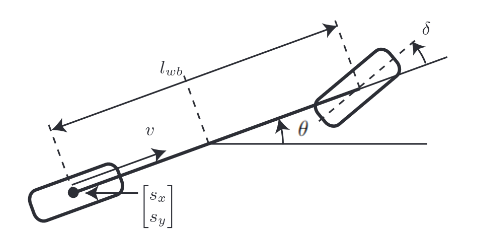
\includegraphics[scale=0.8]{images/kin_model.png}
    \caption{\textit{Kinematic Bicycle Model} con punto di riferimento al centro dell'asse posteriore~\cite{Althoff2017a}.}
    \label{fig:fig10} % etichetta utilizzata per riferisi all'immagine
\end{figure}
Come visibile in Fig.~\ref{fig:fig10}, questa configurazione a due ruote permette di paragonarlo proprio a una \textit{bicicletta}; il modello infatti copre solo il movimento su un piano, 
ignorando di conseguenza i movimenti di rollio e beccheggio. Inoltre, può differire leggermente
a seconda che le variabili di input siano la velocità e la sterzata, o l'accelerazione e la sterzata (come in questo caso).
L'orientamento della ruota anteriore può essere controllato rispetto alla 
direzione del veicolo, mentre non è possibile lo stesso ragionamento
per la ruota posteriore; dunque, di fatto, si considera e si segue solo la ruota anteriore~\cite{Althoff2017a}.

Per formalizzare il \textit{``Kinematic Bicycle Model''}, bisogna 
innanzitutto definire lo spazio degli stati come 
$x=[s_x, s_y, \theta, v]$, dove $s_x$ e $s_y$ sono
le coordinate del veicolo poste al centro dell'asse posteriore, 
$\theta$ è l'orientamento del veicolo e $v$ la velocità; dopodiché, si
definisce il vettore degli input come $u=[a, \delta]$, dove $a$ 
rappresenta l'accelerazione e $\delta$ l'angolo di sterzata delle 
ruote anteriori.
Le equazioni differenziali che descrivono il cambiamento di stato per il modello sono:
\[
\dot{s}_x=v\cos(\theta), \quad
\dot{s}_y=v\sin(\theta), \quad
\dot{v}=a, \quad
\dot{\theta}=\frac{v\tan(\delta)}{l_{wb}}
\]
Dove $l_{wb}$ indica la lunghezza del passo (\textit{wheelbase}) del 
veicolo da una ruota all'altra e corrisponde a 
$l_\text{front} + l_\text{rear}$. 
Le equazioni differenziali indicate sopra si possono esprimere in 
forma sintetica come:
\[ \dot{x} = f(x, u) = A'x + B'u \]
Dove $A'$ e $B'$ sono matrici di sistema continue e, come anticipato, il sistema verrà poi discretizzato (sezione \ref{sect:disc}) e linearizzato (sezione \ref{sect:lin}).

Il modello cinematico ignora l'effetto dello slittamento degli pneumatici e quindi non riflette in 
certi casi la dinamica effettiva~\cite{jain2020bayesrace}. 
In genere, è particolarmente indicato in condizioni di guida normali, tuttavia un modello più 
complesso, come quello dinamico, non necessariamente migliorerebbe le prestazioni poiché potrebbe 
richiedere maggior tempo per la risoluzione. 
Tuttavia, in alcuni casi il modello cinematico può risultare adeguato anche in condizioni di guida 
più estreme; in caso contrario, il modello necessita di una buona rapidità per riuscire a compensare i segnali di controllo non ottimali.

\section{Funzione Obiettivo}
\label{subs:obj}
Il compito della \textit{funzione obiettivo} è quello di assegnare un \textit{costo} $J$
a una traiettoria data, in modo da valutare la bontà di quest'ultima per lo scopo prefissato. 
Considerando $T$ come il numero di passi dell'orizzonte temporale, tale costo può essere espresso come:
\[
\begin{aligned}
J = & \sum_{t=0}^{T}c_t(x_t, u_t) = \\ &
\ Q_{f}\left(x_{T}-x_{T, r e f}\right)^{2}+ \\ & Q \sum_{t=0}^{T-1}\left(x_{t}-x_{t, r e f}\right)^{2}+ \\ & R \sum_{t=0}^{T} u_{t}^{2}+R_{d} \sum_{t=0}^{T-1}\left(u_{t+1}-u_{t}\right)^{2}
\end{aligned}
\]
L'obiettivo consiste nel minimizzare il costo $J$. Si noti che $J$ è quadratica ed è divisa in due parti~\cite{f1tenthcoursel13}:
\begin{enumerate}
    \item \textit{Costo dell'errore di stato}, pesato dalla matrice di peso $Q$ e $Q_f$;
    \item \textit{Costo dell'attuazione}, pesato dalle matrici di peso $R$ e $R_d$. 
\end{enumerate}
Nello specifico, la funzione di costo penalizza sia la differenza tra gli stati calcolati e gli 
stati di riferimento, sia i grandi input di controllo, affinché lo stato desiderato venga 
raggiunto con un input di controllo minimo. Si vogliono infatti minimizzare tre sotto-obiettivi:
\begin{enumerate}
    \item La deviazione del veicolo dalla traiettoria di riferimento: $\forall t \in T, \ x_t-x_{t, r e f}$. 
    La deviazione dello stato finale è pesata da $Q_f$, mentre le altre da $Q$.
    \item Il fattore di influenza degli input di controllo,
    pesato da $R$.
    \item La differenza tra un input di controllo e il successivo, pesata da $R_d$.
\end{enumerate}
Le matrici di pesi $R$, $R_d$ e $Q$ giocano un ruolo fondamentale nel determinare il comportamento
di \textit{MPC}. Esse infatti influenzano il modo in cui l'algoritmo penalizza, rispettivamente, l'attuazione 
degli input di controllo, i cambiamenti negli input di controllo e la deviazione dalla traiettoria di riferimento.
In \textit{MPC}, la matrice $Q$ è sempre semi-definita positiva; ciò garantisce che il costo 
associato agli errori di stato non sia mai negativo, il che è importante per mantenere la 
convessità del problema di ottimizzazione e per garantire che il costo totale non sia appunto negativo.
Invece, la matrice $R$ è sempre definita positiva, garantendo quindi che ci sia sempre un costo associato 
all'applicazione degli input di controllo, evitando così soluzioni banali senza penalità in cui gli input
di controllo potrebbero essere troppo grandi o piccoli. 

Più precisamente, valori più alti per $R$ indicano che l'algoritmo sarà più riluttante a 
utilizzare input di controllo elevati; la matrice $R_d$ può aiutare a ottenere un controllo più 
fluido; infine, le matrici $Q$ e $Q_f$ riducono la deviazione dalla traiettoria di riferimento da seguire.
\section{Vincoli}
Come già anticipato a inizio capitolo, uno dei vantaggi più significativi di \textit{MPC} è 
proprio la possibilità di gestire i \textit{vincoli} del sistema trattato. 
Ciò permette di riflettere in modo più preciso la realtà rispetto a un metodo reattivo come
il \textit{PID Controller}, trattato nel Capitolo~\ref{chap:chap2}.
I vincoli del problema di ottimizzazione sono i seguenti:
\begin{itemize}
    \item lo \textit{stato iniziale} in programma per l'orizzonte corrente deve corrispondere allo 
    stato corrente del veicolo, cioè $x_0 = x(0)$. Quindi, lo stato iniziale $x_0$ è 
    impostato come lo stato corrente del veicolo, mentre il tempo iniziale corrisponde al tempo 
    nello stato di riferimento più vicino allo stato corrente del veicolo.
    \item gli \textit{stati futuri} del veicolo devono seguire il modello della dinamica del veicolo \textit{linearizzato}.
    \item gli \textit{input generati} non devono superare i limiti fisici del veicolo.
\end{itemize}

\subsection{Stati futuri e dinamica}
Un modello che prevede stati $x$ futuri può mutare nel tempo. Alcuni risolutori moderni
possono gestire dinamiche non lineari -- ad esempio \textit{Casadi}, che non è stato però oggetto 
di questo lavoro -- tuttavia spesso si cerca di linearizzare la dinamica del sistema per 
effettuare il calcolo di \textit{MPC} in modo più veloce. La dinamica linearizzata è solitamente nella seguente forma:
\[
x_{t+1} = Ax_t+Bu_t \quad \forall x,u \in [x_0 \ ... \ x_N \ \ \ \ u_0 \ ... \ u_N]^T
\]
% Valutare se usare $k$ o $t$
Questo vincolo su due stati consecutivi, vale a dire $x_t$ e $x_{t+1}$, garantisce che la sequenza 
degli stati possa essere esclusivamente una \textit{traiettoria realistica} che rispetta la 
dinamica del sistema.

\subsection{Stato e input}
I vincoli per stato e input possono essere formulati semplicemente come un limite inferiore e 
superiore su una delle variabili di stato o di controllo.
Alcuni esempi di vincoli di disuguaglianza sono dati da:
\begin{itemize}
    \item \textit{Limiti dell'attuatore} -- in riferimento all'angolo di sterzata, alla velocità, ecc.
    \item \textit{Confini del tracciato} -- può essere interpretato come una regione delimitata da un insieme di linee.
\end{itemize}
Dunque, i vincoli del sistema codificano i domini degli stati
$x_t \in \mathcal{X}$ e degli input $u_t \in \mathcal{U}$ 
consentiti.
Ciascun vincolo di disuguaglianza può essere scritto come $Ax \le b$, dove per ogni riga di $A$, b corrisponde a un vincolo applicato.

\section{Algoritmo}
Si mostra di seguito lo pseudocodice del funzionamento generale dell'algoritmo del 
\textit{Model Predictive Control} che, ricevendo in ingresso la funzione di costo $J$, il modello 
della dinamica del sistema $f$, l'orizzonte degli eventi $T$ e l'input di controllo iniziale
$\hat{u}_0$, risolve all'ottimo il problema.
%\algrenewcommand{\algorithmiccomment}[1]{\hfill// #1}
\begin{algorithm}[H]
\caption{MPC: Model Predictive Control}\label{alg:mpc}
\begin{algorithmic}[1]
\Require Obiettivo $J$, modello della dinamica $f$, orizzonte temporale $T$,
input di controllo iniziale $\hat{u}_0$.
\State $u_t \gets \hat{u}_0$

\While{True}
    \State $x_{0} \gets$ \Call{GET\_CURRENT\_STATE}{}()
    \LComment{Il risolutore viene settato in warm-start, così da sfruttare la soluzione dell'iterazione precedente.}
    \State $u_t \gets$ \Call{SOLVE\_LINEAR\_MPC}{$J, f, x_0, T, u_t$}
    \State $u \gets$ \Call{GET\_FIRST}{$u_t$}
    \State \Call{EXECUTE\_CONTROL}{u}
\EndWhile
\end{algorithmic}
\end{algorithm}
Prima di farlo però, come si può vedere nell'algoritmo~\ref{alg:mpc}, l'input di controllo viene inizializzato con quello iniziale. In 
seguito, dentro il ciclo viene rilevato lo stato corrente $x_0$, che viene poi passato in input al 
risolutore, insieme agli altri componenti principali del problema di ottimizzazione.

Una volta fatto ciò, si ottiene la sequenza di controlli ottimale. Si noti però come l'algoritmo
sfrutta e attua solo il primo di questi input, che corrisponde al primo passo temporale della 
finestra dell'orizzonte data.

Dato che i controlli tra un passo temporale e il successivo variano di poco, si sfrutta il
concetto di \textit{warm start}: si riutilizza l'input di controllo dell'iterazione precedente in 
modo da trovare la soluzione del passo successivo in modo più rapido. In questo modo l'intero 
algoritmo trarrà beneficio da questa caratteristica, richiedendo tempi di calcolo inferiori.

\section{Quadratic Programming}
Il problema di ottimizzazione che caratterizza \textit{MPC} non ha soluzioni analitiche. 
Per poterlo risolvere, infatti, bisogna formulare un problema di
\textit{Quadratic Programming (QP)}. Si tratta di un processo per risolvere problemi di 
ottimizzazione matematica che coinvolgono \textit{funzioni quadratiche}. L'obiettivo di questo 
metodo è quello di trovare un vettore $z$ che minimizzi (o massimizzi) una funzione quadratica 
soggetta a \textit{vincoli lineari} sulle variabili.
Infatti, devono essere mantenute alcune condizioni di frontiera (\textit{boundary}) durante 
l’ottimizzazione, come \textit{lower bound} e \textit{upper bound}. 
In realtà, il termine \textit{``programmazione''} in questo contesto si riferisce solo a una procedura formale usata per risolvere problemi matematici.

Avendo $c,z \in \mathbb{R}^n, A_{m \times n}, Q_{m \times n}$, una forma standard 
comune di \textit{programmazione quadratica} è la seguente:
\[
\begin{aligned}
\min \ f(z) = \frac{1}{2} z^T & Hz + c^Tz \\
\text{subject to } \ & l_b \leq A_c z \leq u_b
\end{aligned}
\]
Un'altra caratteristica di \textit{QP} è che è \textit{convessa}, cioè, esiste un \textit{unico ottimo globale}.
Si ricorda che una funzione a valori reali è detta \textit{convessa} se il segmento di linea che 
congiunge due punti qualsiasi del suo grafico giace sopra il grafico stesso (o coincide con una 
sua parte). In altri termini, se si traccia una linea tra due punti qualsiasi, la funzione sarà sotto la linea.
Inoltre, un problema di questo tipo può essere risolto efficientemente in tempo reale 
(\textit{online}). Sono disponibili molti solutori di QP, tra i quali:
\begin{itemize}
    \item \textit{OSQP}, CVXGen, QuadProg, ecc.
    \item \textit{Casadi} per l’ottimizzazione non convessa.
    \item MPT3 per la progettazione e l'analisi lineare di \textit{MPC}.
\end{itemize}
Il risolutore più consigliato da F1TENTH è \textit{OSQP (Operator Splitting Quadratic Program)}~\cite{osqp}.

Manca ancora un aspetto importante per poter formulare il problema 
come uno di \textit{QP}: bisogna prima \textit{discretizzare} il sistema dinamico 
e \textit{linearizzarlo} attorno a un certo punto.

\subsection{Discretizzazione}
\label{sect:disc}
Per effettuare quest'operazione viene utilizzata -- ma non implementato -- il metodo 
\textit{``Forward Euler''} poiché è il più semplice. Dovrebbero funzionare anche altri metodi, come \textit{RK4/6}.
Per la discretizzazione viene utilizzato il tempo di campionamento $dt$, che può essere scelto come parametro da ottimizzare. 
Si può quindi esprimere l’equazione del sistema come:
\begin{equation}
\label{eq:disc}
x_{t+1} = x_t + f(x_t, u_t) \ dt
\end{equation}

\subsection{Linearizzazione}
\label{sect:lin}
La maggior parte dei sistemi fisici sono non lineari, il che comporta che le loro equazioni sono 
più complesse da risolvere. Invece, i sistemi lineari sono più semplici, sono generalmente ben 
compresi e possono essere analizzati più agevolmente.
I sistemi non lineari possono essere ben approssimati da un sistema lineare in un piccolo intorno 
di un punto presente nello spazio degli \textit{stati}.
L'idea è quella che se il sistema viene controllato per rimanere vicino
a un punto operativo -- in una condizione di lavoro stabile -- si può poi 
sostituire il sistema non lineare con uno linearizzato attorno a quel punto.

Per la \textit{linearizzazione} si sfrutta l’espansione di Taylor del primo 
ordine della funzione a due variabili in (\ref{eq:disc}) attorno a certi $\bar{x}$ e $\bar{u}$, che
porta ad avere: 
\[
\begin{aligned}
x_{t+1}& = \ x_t + (f(\bar{x_t}, \bar{u_t}) + f'_z(\bar{x_t}, \bar{u_t})(x_t - \bar{x_t}) + f'_u(\bar{x_t}, \bar{u_t})(u_t - \bar{u_t}))dt \\
& \rightarrow \ A x_t + B u_t + C
\end{aligned}
\]
Nel contesto di \textit{MPC}, i sistemi lineari consentono di tradurre la dinamica come vincoli 
lineari secondo la formulazione di \textit{MPC}, dunque essi permettono di riscrivere \textit{MPC} come un \textit{QP} standard.
Il problema di ottimizzazione risultante è così di rapida risoluzione.

\subsection{Conversione}
Per passare dalla forma generale del problema di \textit{MPC} alla formulazione 
in programmazione quadratica si effettua principalmente un lavoro di gestione di
indici e di matrici. Per quanto riguarda la funzione di costo $J = \frac{1}{2} z^T H z + c^T z$, vale:
\[
H = \text{diag}(Q, Q, \dots, Q_N, R, \dots, R)
\]
\[
c = \begin{bmatrix}
    -Q x_r \\
    \vdots \\
    -Q_N x_r \\
    0 \\
    \vdots \\
    0
\end{bmatrix}
\quad \quad
z = \begin{bmatrix}
    x_0 \\
    \vdots \\
    x_{N+1} \\
    u_0 \\
    \vdots \\
    u_N
\end{bmatrix}
\]
$H$ è una matrice diagonale in cui ci sono $N-1$ matrici di penalità $Q$ e $N$ matrici $R$ uguali,
dove ognuna di esse fa riferimento a un \textit{timestep} preciso dell'orizzonte di MPC. Si distingue 
solo $Q_N$ perché l'ultima potrebbe avere pesi diversi.
Invece $c$ è un vettore che considera gli stati di riferimento -- dove $-Q x_r$ è 
estratto da $(x_k - x_{ref})^T Q (x_k - x_{ref})$.

Bisogna poi trasformare i vincoli della dinamica e quelli di stato e
input nella forma compatta $l_b \le A_c z \le u_b$. Per la matrice $A_c$, diversamente, si ha:
\[
l_b = \begin{bmatrix}
    -x_0 \\
    0 \\
    \vdots \\
    0 \\
    x_{\text{min}} \\
    \vdots \\
    x_{\text{min}} \\
    u_{\text{min}} \\
    \vdots \\
    u_{\text{min}}
\end{bmatrix}
\quad
A_c = \begin{bmatrix}
    -I & 0 & 0 & \dots & 0 & 0 & 0 & 0 \\
    A & -I & 0 & \dots & 0 & B & 0 & 0 \\
    \vdots & \vdots & \vdots & \ddots & \vdots & \vdots & \vdots & \vdots \\
    \hline
    I & 0 & 0 & \dots & 0 & 0 & 0 & 0 \\
    \vdots & \vdots & \vdots & \ddots & \vdots & \vdots & \vdots & \vdots \\
    0 & 0 & 0 & \dots & 0 & 0 & 0 & I
\end{bmatrix}
\quad
u_b = \begin{bmatrix}
    -x_0 \\
    0 \\
    \vdots \\
    0 \\
    x_{\text{max}} \\
    \vdots \\
    x_{\text{max}} \\
    u_{\text{max}} \\
    \vdots \\
    u_{\text{max}}
\end{bmatrix}
\]
In riferimento alle righe di $A_c$, applicando la forma compatta si ha:
\[
\begin{aligned}
&\text{Riga 1: } -x_0 \le -I x_0 \le -x_0 \ \rightarrow \ x(0) = x_0 & \quad\quad &
\text{stato iniziale} \\
&\text{Riga 2: } \ x_1 = A x_0 + B x_0 & \quad\quad & 
\text{aggiornamento dello stato} \\
&\text{Riga 3: } \ x_{min} \le x \le x_{max} & \quad\quad & 
\text{limiti del stato} \\
&\text{Riga 4: } \ u_{min} \le u \le u_{max} & \quad\quad & \text{limiti del controllo}
\end{aligned}
\]

\section{Vantaggi e svantaggi}
Per concludere, si raggruppano di seguito i punti di forza di \textit{MPC}:
\begin{enumerate}
    \item È un controller ad alte prestazioni che gestisce sistematicamente i vincoli.
    \item Considera preventivamente le decisioni future. 
    \item Ha una formulazione flessibile che può incorporare sotto-obiettivi aggiuntivi.
    \item Può essere formulato anche per la dinamica dei sistemi non lineari.
    \item È in grado di gestire anche dinamiche variabili nel tempo.
\end{enumerate}
La sfida principale quando si implementa \textit{MPC} è il carico 
computazionale causato dalla risoluzione in tempo reale
del problema di ottimizzazione, ripetuta per ogni passo temporale. I principali fattori che 
influenzano il tempo di calcolo sono il numero di \textit{stati}, il numero di \textit{input} e 
l’orizzonte di previsione~\cite{hierarchmpc}. Ci sono poi anche altre sfide da affrontare per 
raggiungere buone performance, poiché l'algoritmo non riesce sempre a garantire la stabilità, la praticabilità e la robustezza.